% Options for packages loaded elsewhere
\PassOptionsToPackage{unicode}{hyperref}
\PassOptionsToPackage{hyphens}{url}
%
\documentclass[
]{article}
\usepackage{amsmath,amssymb}
\usepackage{iftex}
\ifPDFTeX
  \usepackage[T1]{fontenc}
  \usepackage[utf8]{inputenc}
  \usepackage{textcomp} % provide euro and other symbols
\else % if luatex or xetex
  \usepackage{unicode-math} % this also loads fontspec
  \defaultfontfeatures{Scale=MatchLowercase}
  \defaultfontfeatures[\rmfamily]{Ligatures=TeX,Scale=1}
\fi
\usepackage{lmodern}
\ifPDFTeX\else
  % xetex/luatex font selection
\fi
% Use upquote if available, for straight quotes in verbatim environments
\IfFileExists{upquote.sty}{\usepackage{upquote}}{}
\IfFileExists{microtype.sty}{% use microtype if available
  \usepackage[]{microtype}
  \UseMicrotypeSet[protrusion]{basicmath} % disable protrusion for tt fonts
}{}
\makeatletter
\@ifundefined{KOMAClassName}{% if non-KOMA class
  \IfFileExists{parskip.sty}{%
    \usepackage{parskip}
  }{% else
    \setlength{\parindent}{0pt}
    \setlength{\parskip}{6pt plus 2pt minus 1pt}}
}{% if KOMA class
  \KOMAoptions{parskip=half}}
\makeatother
\usepackage{xcolor}
\usepackage[margin=1in]{geometry}
\usepackage{color}
\usepackage{fancyvrb}
\newcommand{\VerbBar}{|}
\newcommand{\VERB}{\Verb[commandchars=\\\{\}]}
\DefineVerbatimEnvironment{Highlighting}{Verbatim}{commandchars=\\\{\}}
% Add ',fontsize=\small' for more characters per line
\usepackage{framed}
\definecolor{shadecolor}{RGB}{248,248,248}
\newenvironment{Shaded}{\begin{snugshade}}{\end{snugshade}}
\newcommand{\AlertTok}[1]{\textcolor[rgb]{0.94,0.16,0.16}{#1}}
\newcommand{\AnnotationTok}[1]{\textcolor[rgb]{0.56,0.35,0.01}{\textbf{\textit{#1}}}}
\newcommand{\AttributeTok}[1]{\textcolor[rgb]{0.13,0.29,0.53}{#1}}
\newcommand{\BaseNTok}[1]{\textcolor[rgb]{0.00,0.00,0.81}{#1}}
\newcommand{\BuiltInTok}[1]{#1}
\newcommand{\CharTok}[1]{\textcolor[rgb]{0.31,0.60,0.02}{#1}}
\newcommand{\CommentTok}[1]{\textcolor[rgb]{0.56,0.35,0.01}{\textit{#1}}}
\newcommand{\CommentVarTok}[1]{\textcolor[rgb]{0.56,0.35,0.01}{\textbf{\textit{#1}}}}
\newcommand{\ConstantTok}[1]{\textcolor[rgb]{0.56,0.35,0.01}{#1}}
\newcommand{\ControlFlowTok}[1]{\textcolor[rgb]{0.13,0.29,0.53}{\textbf{#1}}}
\newcommand{\DataTypeTok}[1]{\textcolor[rgb]{0.13,0.29,0.53}{#1}}
\newcommand{\DecValTok}[1]{\textcolor[rgb]{0.00,0.00,0.81}{#1}}
\newcommand{\DocumentationTok}[1]{\textcolor[rgb]{0.56,0.35,0.01}{\textbf{\textit{#1}}}}
\newcommand{\ErrorTok}[1]{\textcolor[rgb]{0.64,0.00,0.00}{\textbf{#1}}}
\newcommand{\ExtensionTok}[1]{#1}
\newcommand{\FloatTok}[1]{\textcolor[rgb]{0.00,0.00,0.81}{#1}}
\newcommand{\FunctionTok}[1]{\textcolor[rgb]{0.13,0.29,0.53}{\textbf{#1}}}
\newcommand{\ImportTok}[1]{#1}
\newcommand{\InformationTok}[1]{\textcolor[rgb]{0.56,0.35,0.01}{\textbf{\textit{#1}}}}
\newcommand{\KeywordTok}[1]{\textcolor[rgb]{0.13,0.29,0.53}{\textbf{#1}}}
\newcommand{\NormalTok}[1]{#1}
\newcommand{\OperatorTok}[1]{\textcolor[rgb]{0.81,0.36,0.00}{\textbf{#1}}}
\newcommand{\OtherTok}[1]{\textcolor[rgb]{0.56,0.35,0.01}{#1}}
\newcommand{\PreprocessorTok}[1]{\textcolor[rgb]{0.56,0.35,0.01}{\textit{#1}}}
\newcommand{\RegionMarkerTok}[1]{#1}
\newcommand{\SpecialCharTok}[1]{\textcolor[rgb]{0.81,0.36,0.00}{\textbf{#1}}}
\newcommand{\SpecialStringTok}[1]{\textcolor[rgb]{0.31,0.60,0.02}{#1}}
\newcommand{\StringTok}[1]{\textcolor[rgb]{0.31,0.60,0.02}{#1}}
\newcommand{\VariableTok}[1]{\textcolor[rgb]{0.00,0.00,0.00}{#1}}
\newcommand{\VerbatimStringTok}[1]{\textcolor[rgb]{0.31,0.60,0.02}{#1}}
\newcommand{\WarningTok}[1]{\textcolor[rgb]{0.56,0.35,0.01}{\textbf{\textit{#1}}}}
\usepackage{graphicx}
\makeatletter
\def\maxwidth{\ifdim\Gin@nat@width>\linewidth\linewidth\else\Gin@nat@width\fi}
\def\maxheight{\ifdim\Gin@nat@height>\textheight\textheight\else\Gin@nat@height\fi}
\makeatother
% Scale images if necessary, so that they will not overflow the page
% margins by default, and it is still possible to overwrite the defaults
% using explicit options in \includegraphics[width, height, ...]{}
\setkeys{Gin}{width=\maxwidth,height=\maxheight,keepaspectratio}
% Set default figure placement to htbp
\makeatletter
\def\fps@figure{htbp}
\makeatother
\setlength{\emergencystretch}{3em} % prevent overfull lines
\providecommand{\tightlist}{%
  \setlength{\itemsep}{0pt}\setlength{\parskip}{0pt}}
\setcounter{secnumdepth}{-\maxdimen} % remove section numbering
\ifLuaTeX
  \usepackage{selnolig}  % disable illegal ligatures
\fi
\usepackage{bookmark}
\IfFileExists{xurl.sty}{\usepackage{xurl}}{} % add URL line breaks if available
\urlstyle{same}
\hypersetup{
  pdftitle={Coding\_Challenge\_DataWrangling},
  pdfauthor={Pankaj Gaonkar},
  hidelinks,
  pdfcreator={LaTeX via pandoc}}

\title{Coding\_Challenge\_DataWrangling}
\author{Pankaj Gaonkar}
\date{2025-03-20}

\begin{document}
\maketitle

\section{Coding Challenge \_ Data
Wrangling}\label{coding-challenge-_-data-wrangling}

\begin{Shaded}
\begin{Highlighting}[]
\CommentTok{\#install.packages("tidyverse")}
\FunctionTok{library}\NormalTok{(tidyverse)}
\end{Highlighting}
\end{Shaded}

\begin{verbatim}
## Warning: package 'ggplot2' was built under R version 4.4.3
\end{verbatim}

\begin{verbatim}
## Warning: package 'purrr' was built under R version 4.4.2
\end{verbatim}

\begin{verbatim}
## Warning: package 'lubridate' was built under R version 4.4.2
\end{verbatim}

\begin{verbatim}
## -- Attaching core tidyverse packages ------------------------ tidyverse 2.0.0 --
## v dplyr     1.1.4     v readr     2.1.5
## v forcats   1.0.0     v stringr   1.5.1
## v ggplot2   3.5.1     v tibble    3.2.1
## v lubridate 1.9.4     v tidyr     1.3.1
## v purrr     1.0.4     
## -- Conflicts ------------------------------------------ tidyverse_conflicts() --
## x dplyr::filter() masks stats::filter()
## x dplyr::lag()    masks stats::lag()
## i Use the conflicted package (<http://conflicted.r-lib.org/>) to force all conflicts to become errors
\end{verbatim}

\section{1. 3 pts. Download two .csv files from Canvas called
DiversityData.csv and Metadata.csv, and read them into R using relative
file
paths.}\label{pts.-download-two-.csv-files-from-canvas-called-diversitydata.csv-and-metadata.csv-and-read-them-into-r-using-relative-file-paths.}

\begin{Shaded}
\begin{Highlighting}[]
\NormalTok{DiversityData }\OtherTok{\textless{}{-}} \FunctionTok{read.csv}\NormalTok{(}\StringTok{"DiversityData.csv"}\NormalTok{)}
\FunctionTok{str}\NormalTok{(DiversityData)}
\end{Highlighting}
\end{Shaded}

\begin{verbatim}
## 'data.frame':    70 obs. of  5 variables:
##  $ Code      : chr  "S01_13" "S02_16" "S03_19" "S04_22" ...
##  $ shannon   : num  6.62 6.61 6.66 6.66 6.61 ...
##  $ invsimpson: num  211 207 213 205 200 ...
##  $ simpson   : num  0.995 0.995 0.995 0.995 0.995 ...
##  $ richness  : int  3319 3079 3935 3922 3196 3481 3250 3170 3657 3177 ...
\end{verbatim}

\begin{Shaded}
\begin{Highlighting}[]
\NormalTok{Metadata }\OtherTok{\textless{}{-}} \FunctionTok{read.csv}\NormalTok{(}\StringTok{"Metadata.csv"}\NormalTok{)}

\FunctionTok{str}\NormalTok{(Metadata)}
\end{Highlighting}
\end{Shaded}

\begin{verbatim}
## 'data.frame':    70 obs. of  5 variables:
##  $ Code         : chr  "S01_13" "S02_16" "S03_19" "S04_22" ...
##  $ Crop         : chr  "Soil" "Soil" "Soil" "Soil" ...
##  $ Time_Point   : int  0 0 0 0 0 0 6 6 6 6 ...
##  $ Replicate    : int  1 2 3 4 5 6 1 2 3 4 ...
##  $ Water_Imbibed: chr  "na" "na" "na" "na" ...
\end{verbatim}

\section{2. 4 pts. Join the two dataframes together by the common column
`Code'. Name the resulting dataframe
alpha.}\label{pts.-join-the-two-dataframes-together-by-the-common-column-code.-name-the-resulting-dataframe-alpha.}

\begin{Shaded}
\begin{Highlighting}[]
\NormalTok{alpha  }\OtherTok{\textless{}{-}} \FunctionTok{left\_join}\NormalTok{(Metadata, DiversityData, }\AttributeTok{by =} \StringTok{"Code"}\NormalTok{)}
\end{Highlighting}
\end{Shaded}

\section{3. 4 pts. Calculate Pielou's evenness index: Pielou's evenness
is an ecological parameter calculated by the Shannon diversity index
(column Shannon) divided by the log of the richness
column.}\label{pts.-calculate-pielous-evenness-index-pielous-evenness-is-an-ecological-parameter-calculated-by-the-shannon-diversity-index-column-shannon-divided-by-the-log-of-the-richness-column.}

\#a. Using mutate, create a new column to calculate Pielou's evenness
index. \#b. Name the resulting dataframe alpha\_even.

\begin{Shaded}
\begin{Highlighting}[]
\CommentTok{\# Creating a new column}
\NormalTok{alpha\_even  }\OtherTok{\textless{}{-}}  \FunctionTok{mutate}\NormalTok{(alpha, }\AttributeTok{Pielou\_eveness =}\NormalTok{ shannon }\SpecialCharTok{/} \FunctionTok{log}\NormalTok{(richness))}
\end{Highlighting}
\end{Shaded}

\section{4 4. Pts. Using tidyverse language of functions and the pipe,
use the summarise function and tell me the mean and standard error
evenness grouped by crop over
time.}\label{pts.-using-tidyverse-language-of-functions-and-the-pipe-use-the-summarise-function-and-tell-me-the-mean-and-standard-error-evenness-grouped-by-crop-over-time.}

\#a. Start with the alpha\_even dataframe \#b. Group the data: group the
data by Crop and Time\_Point. \#c.~Summarize the data: Calculate the
mean, count, standard deviation, and standard error for the even
variable within each group. \#d.~Name the resulting dataframe
alpha\_average

\begin{Shaded}
\begin{Highlighting}[]
\CommentTok{\#summary statistics}

\NormalTok{alpha\_average  }\OtherTok{\textless{}{-}}\NormalTok{  alpha\_even }\SpecialCharTok{\%\textgreater{}\%}
    \FunctionTok{group\_by}\NormalTok{(Crop, Time\_Point) }\SpecialCharTok{\%\textgreater{}\%}
    \FunctionTok{summarise}\NormalTok{(}\AttributeTok{mean.even =} \FunctionTok{mean}\NormalTok{(Pielou\_eveness), }\CommentTok{\# calculating the mean richness, stdeviation, and standard error}
            \AttributeTok{n =} \FunctionTok{n}\NormalTok{(), }
            \AttributeTok{sd.dev =} \FunctionTok{sd}\NormalTok{(Pielou\_eveness)) }\SpecialCharTok{\%\textgreater{}\%}
    \FunctionTok{mutate}\NormalTok{(}\AttributeTok{std.err =}\NormalTok{ sd.dev}\SpecialCharTok{/}\FunctionTok{sqrt}\NormalTok{(n))}
\end{Highlighting}
\end{Shaded}

\begin{verbatim}
## `summarise()` has grouped output by 'Crop'. You can override using the
## `.groups` argument.
\end{verbatim}

\section{5. 4. Pts. Calculate the difference between the soybean column,
the soil column, and the difference between the cotton column and the
soil
column}\label{pts.-calculate-the-difference-between-the-soybean-column-the-soil-column-and-the-difference-between-the-cotton-column-and-the-soil-column}

\#a. Start with the alpha\_average dataframe \#b. Select relevant
columns: select the columns Time\_Point, Crop, and mean.even.
\#c.~Reshape the data: Use the pivot\_wider function to transform the
data from long to wide format, creating new columns for each Crop with
values from mean.even. \#d.~Calculate differences: Create new columns
named diff.cotton.even and diff.soybean.even by calculating the
difference between Soil and Cotton, and Soil and Soybean, respectively.
\#e. Name the resulting dataframe alpha\_average2

\begin{Shaded}
\begin{Highlighting}[]
\NormalTok{alpha\_average2 }\OtherTok{\textless{}{-}}\NormalTok{ alpha\_average }\SpecialCharTok{\%\textgreater{}\%}
              \FunctionTok{select}\NormalTok{(Time\_Point, Crop, mean.even) }\SpecialCharTok{\%\textgreater{}\%}
              \FunctionTok{pivot\_wider}\NormalTok{(}\AttributeTok{names\_from =}\NormalTok{ Crop, }\AttributeTok{values\_from =}\NormalTok{ mean.even) }\SpecialCharTok{\%\textgreater{}\%}
              \FunctionTok{mutate}\NormalTok{(}\AttributeTok{diff.cotton.even =}\NormalTok{ Soil }\SpecialCharTok{{-}}\NormalTok{ Cotton) }\SpecialCharTok{\%\textgreater{}\%}
              \FunctionTok{mutate}\NormalTok{(}\AttributeTok{diff.soybean.even =}\NormalTok{ Soil }\SpecialCharTok{{-}}\NormalTok{ Soybean)}
\end{Highlighting}
\end{Shaded}

\section{6. 4 pts. Connecting it to
plots}\label{pts.-connecting-it-to-plots}

\#a. Start with the alpha\_average2 dataframe \#b. Select relevant
columns: select the columns Time\_Point, diff.cotton.even, and
diff.soybean.even. \#c.~Reshape the data: Use the pivot\_longer function
to transform the data from wide to long format, creating a new column
named diff that contains the values from diff.cotton.even and
diff.soybean.even. \#i. This might be challenging, so I'll give you a
break. The code is below.

\#pivot\_longer(c(diff.cotton.even, diff.soybean.even), names\_to =
``diff'')

\#d.~Create the plot: Use ggplot and geom\_line() with `Time\_Point' on
the x-axis, the column `values' on the y-axis, and different colors for
each `diff' category. The column named `values' come from the
pivot\_longer. The resulting plot should look like the one to the right.

\begin{Shaded}
\begin{Highlighting}[]
\NormalTok{alpha\_average2 }\SpecialCharTok{\%\textgreater{}\%}
  \FunctionTok{select}\NormalTok{(Time\_Point, diff.cotton.even, diff.soybean.even) }\SpecialCharTok{\%\textgreater{}\%}
  \FunctionTok{pivot\_longer}\NormalTok{(}\FunctionTok{c}\NormalTok{(diff.cotton.even, diff.soybean.even), }\AttributeTok{names\_to =} \StringTok{"diff"}\NormalTok{) }\SpecialCharTok{\%\textgreater{}\%}
  \FunctionTok{ggplot}\NormalTok{(}\FunctionTok{aes}\NormalTok{(}\AttributeTok{x =}\NormalTok{ Time\_Point, }\AttributeTok{y =}\NormalTok{ value, }\AttributeTok{color=}\NormalTok{diff)) }\SpecialCharTok{+} \CommentTok{\# Plot it }
  \FunctionTok{geom\_line}\NormalTok{() }\SpecialCharTok{+}
  \FunctionTok{theme\_minimal}\NormalTok{() }\SpecialCharTok{+}
  \FunctionTok{xlab}\NormalTok{(}\StringTok{"Time (hrs)"}\NormalTok{) }\SpecialCharTok{+}
  \FunctionTok{ylab}\NormalTok{(}\StringTok{"Difference from soil in Pielou’s evenness"}\NormalTok{)}
\end{Highlighting}
\end{Shaded}

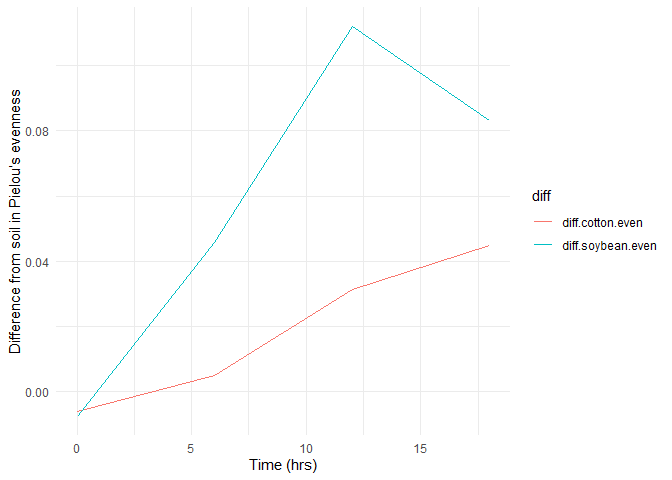
\includegraphics{Coding_challenge_DataWrangling_files/figure-latex/unnamed-chunk-6-1.pdf}

\subsection{Below is the clickable link to GitHub Folder where these
files are
published}\label{below-is-the-clickable-link-to-github-folder-where-these-files-are-published}

\href{https://github.com/ppg0001/PLPA_Assignment/tree/main/Coding_challenge_5}{Coding\_challenge\_5
Folder}

\end{document}
